\subsubsection{Support Vector Machine}

Posterior al tiempo de búsqueda de parámetros del \textit{GridSearchCV} para el modelo de \textit{Support Vector Classifier}, se ejecutó la siguiente celda de código para saber los parámetros con mejor desempeño entre los propuestos: \\

\lstset{
    language=Python,
    basicstyle=\ttfamily\footnotesize,
    keywordstyle=\color{blue},
    commentstyle=\color{gray},
    stringstyle=\color{green!60!black},
    numberstyle=\tiny\color{gray},
    numbers=left,
    breaklines=true,
    frame=single,
    captionpos=b,
    tabsize=4,
    showspaces=false,
    showstringspaces=false,
    showtabs=false
}

\begin{lstlisting}[caption={Código para impresión de parámetros con mejor desempeño y evaluación del modelo}]
# Imprimir parametros con mejores metricas
print(f'Best C: {grid_search.best_params_["C"]}')
print(f'Best kernel: {grid_search.best_params_["kernel"]}')
print(f'Best gamma: {grid_search.best_params_["gamma"]}')

# Evaluar el modelo con los mejores parametros
best_svm_model = grid_search.best_estimator_
y_pred = best_svm_model.predict(X_test)
accuracy = accuracy_score(Y_test, y_pred)
print(f'Precision con el mejor C, kernel y gamma: {accuracy:.2f}')
\end{lstlisting}

\lstset{
    basicstyle=\ttfamily\footnotesize,    % Mantener la fuente monoespaciada
    backgroundcolor=\color{white},        % Fondo blanco
    keywordstyle=\color{black},           % Palabras clave en negro
    commentstyle=\color{black},           % Comentarios en negro
    stringstyle=\color{black}             % Cadenas en negro
}

\begin{lstlisting}[caption={Impresión mejores parámetros y evaluación del modelo}]
Best C: 10
Best kernel: rbf
Best gamma: 0.01
Precision con el mejor C, kernel y gamma: 0.87
\end{lstlisting}

Se graficó la matriz de confusión con ayuda de la función \textit{confusion\_matrix} alojada en la librería \textit{sklearn.metrics} y con apoyo de la librería \textit{seaborn}, obteniendo el resultado siguiente:

\begin{figure}[H]
    \centering
    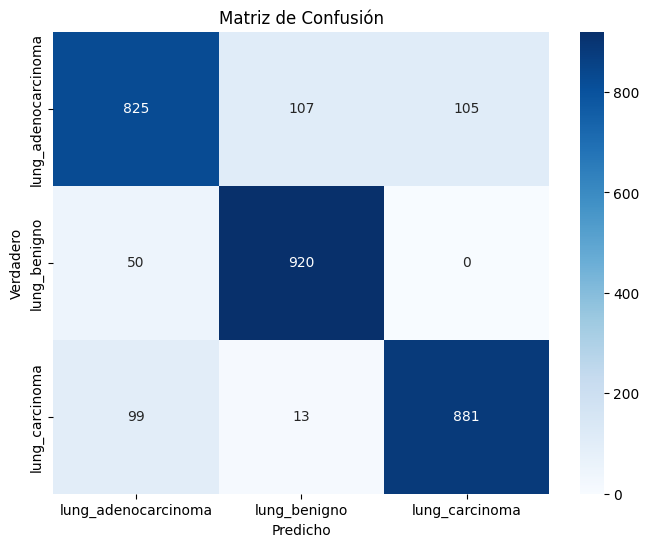
\includegraphics[width=0.65\textwidth]{Francisco/Imagenes resultados/CMSVM.png} 
    \caption{Matriz de confusión del modelo de \textit{SVC}}
\end{figure}

Como última métrica para este modelo se generó el reporte de clasificación con ayuda de la función \textit{classification\_report} alojada igualmente en la librería \textit{sklearn.metrics}:

\begin{table}[H]
    \centering
    \begin{tabular}{l c c c c}

         & precision & recall & f1-score & support \\
        \\
        lung\_adenocarcinoma & 0.85 & 0.80 & 0.82 & 1037 \\
        lung\_benigno & 0.88 & 0.95 & 0.92 & 970 \\
        lung\_carcinoma & 0.89 & 0.89 & 0.89 & 993 \\
        \\
        accuracy &  &  & 0.88 & 3000 \\
        macro avg & 0.88 & 0.88 & 0.88 & 3000 \\
        weighted avg & 0.87 & 0.88 & 0.87 & 3000
        
    \end{tabular}
    \caption{Reporte de clasificación del modelo de \textit{SVC}}
\end{table}

\subsubsection{Regresión Logística}

Tras el tiempo de búsqueda de los mejores parámetros del \textit{GridSearchCV} para el modelo de Regresión Logística, se ejecutó la siguiente celda de código para saber los parámetros con mejor desempeño, de los dados al \textit{GridSearchCV}: \\

\lstset{
    language=Python,
    basicstyle=\ttfamily\footnotesize,
    keywordstyle=\color{blue},
    commentstyle=\color{gray},
    stringstyle=\color{green!60!black},
    numberstyle=\tiny\color{gray},
    numbers=left,
    breaklines=true,
    frame=single,
    captionpos=b,
    tabsize=4,
    showspaces=false,
    showstringspaces=false,
    showtabs=false
}

\begin{lstlisting}[caption={Código para impresión de parámetros con mejor desempeño y evaluación del modelo}]
# Imprimir lista de mejores parametros
print("Mejores parametros encontrados: ", grid_search_lrm.best_params_)
# Imprimir precision del modelo con mejores parametros
print("Mejor precision obtenida: ", grid_search_lrm.best_score_)
\end{lstlisting}

\lstset{
    basicstyle=\ttfamily\footnotesize,    % Mantener la fuente monoespaciada
    backgroundcolor=\color{white},        % Fondo blanco
    keywordstyle=\color{black},           % Palabras clave en negro
    commentstyle=\color{black},           % Comentarios en negro
    stringstyle=\color{black}             % Cadenas en negro
}

\begin{lstlisting}[caption={Impresión mejores parámetros y evaluación del modelo}]
Mejores parametros encontrados:  {'C': 0.01, 'penalty': 'l2', 'solver': 'lbfgs'}
Mejor precision obtenida:  0.6869166666666666
\end{lstlisting}

Se graficó la matriz de confusión del modelo de regresión logística usando las mismas librerías, obteniendo la gráfica siguiente:

\begin{figure}[H]
    \centering
    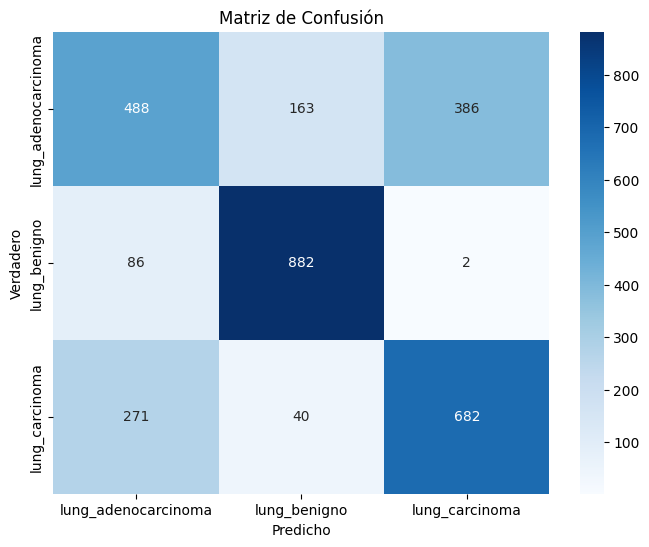
\includegraphics[width=0.65\textwidth]{Francisco/Imagenes resultados/CMLR.png} 
    \caption{Matriz de confusión del modelo de Regresión Logística}
\end{figure}

Como última métrica del modelo de regresión logística se generó el reporte de clasificación, obteniendo el resultado siguiente: 

\begin{table}[H]
    \centering
    \begin{tabular}{l c c c c}

         & precision & recall & f1-score & support \\
        \\
        lung\_adenocarcinoma & 0.58 & 0.47 & 0.52 & 1037 \\
        lung\_benigno & 0.81 & 0.91 & 0.86 & 970 \\
        lung\_carcinoma & 0.64 & 0.69 & 0.66 & 993 \\
        \\
        accuracy &  &  & 0.68 & 3000 \\
        macro avg & 0.68 & 0.69 & 0.68 & 3000 \\
        weighted avg & 0.67 & 0.68 & 0.68 & 3000
        
    \end{tabular}
    \caption{Reporte de clasificación del modelo de Regresión Logística}
\end{table}

\subsubsection{XGBClassifier}

Luego de una extensa búsqueda del \textit{GridSearchCV} con el modelo \textit{XGBClassifier}, se ejecutó la siguiente celda de código para saber los parámetros del modelo con mejor desempeño:

\lstset{
    language=Python,
    basicstyle=\ttfamily\footnotesize,
    keywordstyle=\color{blue},
    commentstyle=\color{gray},
    stringstyle=\color{green!60!black},
    numberstyle=\tiny\color{gray},
    numbers=left,
    breaklines=true,
    frame=single,
    captionpos=b,
    tabsize=4,
    showspaces=false,
    showstringspaces=false,
    showtabs=false
}

\begin{lstlisting}[caption={Código para impresión de parámetros con mejor desempeño y evaluación del modelo}]
# Imprimir parametros con mejores metricas
print(f'Best n_estimators: {grid_search_XGB.best_params_["n_estimators"]}')
print(f'Best learning_rate: {grid_search_XGB.best_params_["learning_rate"]}')
print(f'Best max_depth: {grid_search_XGB.best_params_["max_depth"]}')
print(f'Best subsample: {grid_search_XGB.best_params_["subsample"]}')
print(f'Best colsample_bytree: {grid_search_XGB.best_params_["colsample_bytree"]}')
print(f'Best gamma: {grid_search_XGB.best_params_["gamma"]}')
print(f'Best reg_alpha: {grid_search_XGB.best_params_["reg_alpha"]}')
print(f'Best reg_lambda: {grid_search_XGB.best_params_["reg_lambda"]}')

# Evaluar el modelo con los mejores parametros
best_XGB_model = grid_search_XGB.best_estimator_
y_pred = best_XGB_model.predict(X_test)
accuracy = accuracy_score(Y_test, y_pred)
print(f'Precision con los mejores parametros: {accuracy:.2f}')
\end{lstlisting}

\lstset{
    basicstyle=\ttfamily\footnotesize,    % Mantener la fuente monoespaciada
    backgroundcolor=\color{white},        % Fondo blanco
    keywordstyle=\color{black},           % Palabras clave en negro
    commentstyle=\color{black},           % Comentarios en negro
    stringstyle=\color{black}             % Cadenas en negro
}

\begin{lstlisting}[caption={Impresión mejores parámetros y evaluación del modelo}]
Best n_estimators: 200
Best learning_rate: 0.1
Best max_depth: 10
Best subsample: 0.7
Best colsample_bytree: 0.7
Best gamma: 0.1
Best reg_alpha: 0.1
Best reg_lambda: 10
Precision con los mejores parametros: 0.90
\end{lstlisting}

Se graficó la matriz de confusión del modelo \textit{XGBClassifier}, obteniendo la gráfica siguiente: \\

\begin{figure}[H]
    \centering
    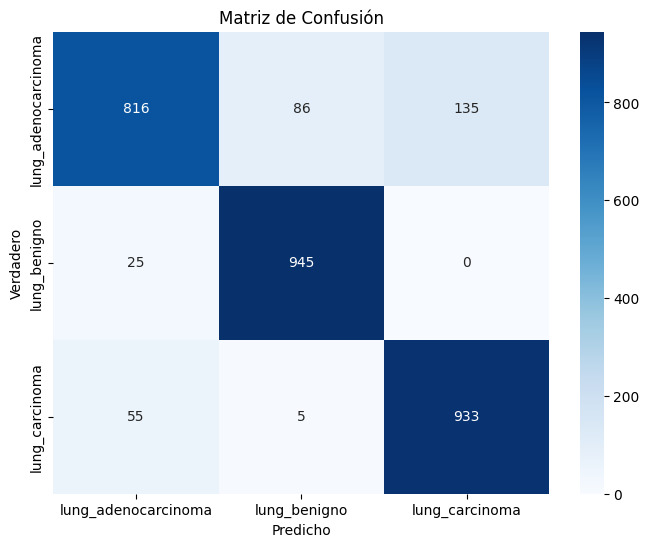
\includegraphics[width=0.65\textwidth]{Francisco/Imagenes resultados/CMXGB.jpeg} 
    \caption{Matriz de confusión del modelo de \textit{XGBCLassifier}}
\end{figure}

Y nuevamente como última métrica del modelo, se generó el reporte de clasificación generando lo siguiente:

\begin{table}[H]
    \centering
    \begin{tabular}{l c c c c}

         & precision & recall & f1-score & support \\
        \\
        lung\_adenocarcinoma & 0.91 & 0.79 & 0.84 & 1037 \\
        lung\_benigno & 0.91 & 0.97 & 0.94 & 970 \\
        lung\_carcinoma & 0.87 & 0.94 & 0.91 & 993 \\
        \\
        accuracy &  &  & 0.90 & 3000 \\
        macro avg & 0.90 & 0.90 & 0.90 & 3000 \\
        weighted avg & 0.90 & 0.90 & 0.90 & 3000
    
    \end{tabular}
    \caption{Reporte de clasificación del modelo \textit{XGBClassifier}}
\end{table}

\newpage

\subsubsection{\textit{Transfer Learning} con \textit{MobileNetV2}}

Este modelo tardó 22 épocas en entrenarse. Se ejecutó la siguiente celda de código para medir el \textit{accuracy} del modelo:

\lstset{
    language=Python,
    basicstyle=\ttfamily\footnotesize,
    keywordstyle=\color{blue},
    commentstyle=\color{gray},
    stringstyle=\color{green!60!black},
    numberstyle=\tiny\color{gray},
    numbers=left,
    breaklines=true,
    frame=single,
    captionpos=b,
    tabsize=4,
    showspaces=false,
    showstringspaces=false,
    showtabs=false
}

\begin{lstlisting}[caption={Código para la impresión del \textit{accuracy} del modelo}]
# Evaluamos el modelo
loss, accuracy = model.evaluate(val_ds)
print(f"Accuracy: {accuracy}")
\end{lstlisting}

\lstset{
    basicstyle=\ttfamily\footnotesize,    % Mantener la fuente monoespaciada
    backgroundcolor=\color{white},        % Fondo blanco
    keywordstyle=\color{black},           % Palabras clave en negro
    commentstyle=\color{black},           % Comentarios en negro
    stringstyle=\color{black}             % Cadenas en negro
}

\begin{lstlisting}[caption={Impresión \textit{accuracy} del modelo}]
Accuracy: 0.9940000176429749
\end{lstlisting}

Para los modelos CNN, se generaron adicionalmente las gráficas de \textit{Training vs Validation} para las medidas \textit{accuracy} y \textit{loss}. Esto con apoyo del método \textit{history} aplicado al modelo entrenado, estos fueron los resultados: 

\begin{figure}[H]
    \centering
    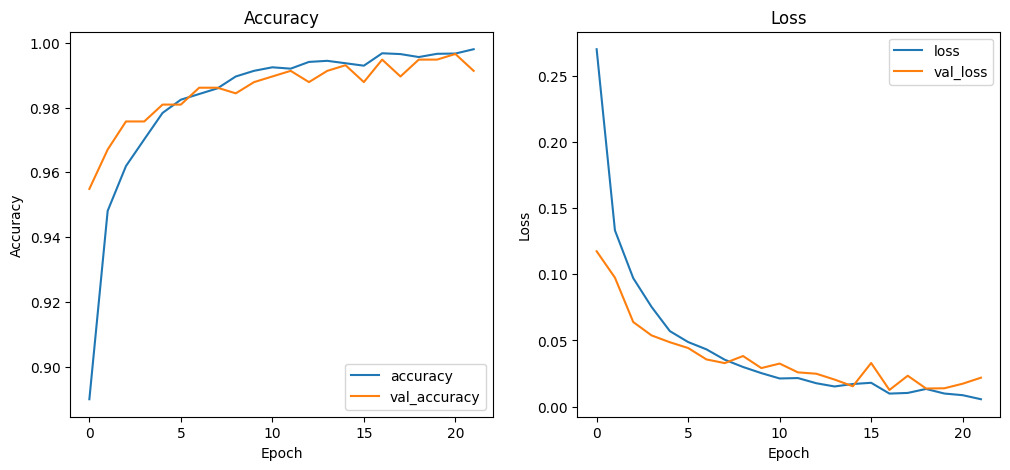
\includegraphics[width=0.85\textwidth]{Francisco/Imagenes resultados/TvsV1.jpeg} 
    \caption{Gráfica \textit{Training vs Validation} de modelo \textit{Transfer Learning} con \textit{MobileNetV2}}
\end{figure}

Al ser un modelo de clasificación, se generó igualmente una matriz de confusión con las predicciones del modelo y se obtuvo la gráfica siguiente:

\begin{figure}[H]
    \centering
    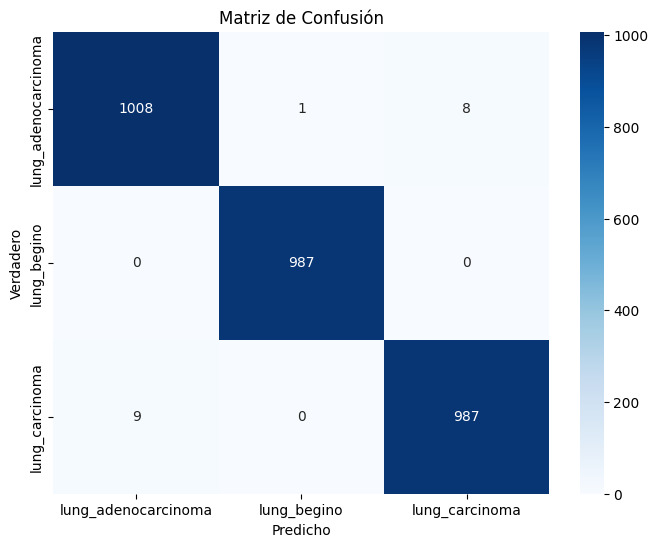
\includegraphics[width=0.60\textwidth]{Francisco/Imagenes resultados/CMCNN1.jpeg} 
    \caption{Matriz de confusión de modelo \textit{Transfer Learning} con \textit{MobileNetV2}}
\end{figure}

Una vez más se generó el reporte de clasificación, el resultado fue el siguiente:

\begin{table}[H]
    \centering
    \begin{tabular}{l c c c c}

         & precision & recall & f1-score & support \\
        \\
        lung\_adenocarcinoma & 0.99 & 0.99 & 0.99 & 1017 \\
        lung\_benigno & 1.00 & 1.00 & 1.00 & 987 \\
        lung\_carcinoma & 0.99 & 0.99 & 0.99 & 996 \\
        \\
        accuracy &  &  & 0.99 & 3000 \\
        macro avg & 0.99 & 0.99 & 0.99 & 3000 \\
        weighted avg & 0.99 & 0.99 & 0.99 & 3000
    
    \end{tabular}
    \caption{Reporte de clasificación de modelo \textit{Transfer Learning} con \textit{MobileNetV2}}
\end{table}

\subsubsection{\textit{Transfer Learning} con \textit{VGG16}}

Este modelo tardó 31 épocas en entrenarse. Se ejecutó la siguiente celda de código para medir el \textit{accuracy} del modelo:

\lstset{
    language=Python,
    basicstyle=\ttfamily\footnotesize,
    keywordstyle=\color{blue},
    commentstyle=\color{gray},
    stringstyle=\color{green!60!black},
    numberstyle=\tiny\color{gray},
    numbers=left,
    breaklines=true,
    frame=single,
    captionpos=b,
    tabsize=4,
    showspaces=false,
    showstringspaces=false,
    showtabs=false
}

\begin{lstlisting}[caption={Código para la impresión del \textit{accuracy} del modelo}]
# Evaluamos el modelo
loss, accuracy = model.evaluate(val_ds)
print(f"Accuracy: {accuracy}")
\end{lstlisting}

\lstset{
    basicstyle=\ttfamily\footnotesize,    % Mantener la fuente monoespaciada
    backgroundcolor=\color{white},        % Fondo blanco
    keywordstyle=\color{black},           % Palabras clave en negro
    commentstyle=\color{black},           % Comentarios en negro
    stringstyle=\color{black}             % Cadenas en negro
}

\begin{lstlisting}[caption={Impresión \textit{accuracy} del modelo}]
Accuracy: 0.9660000205039978
\end{lstlisting}

Las gráficas de \textit{Training vs Validation} para las medidas de \textit{accuracy} y \textit{loss}, fueron las siguientres para este modelo: 

\begin{figure}[H]
    \centering
    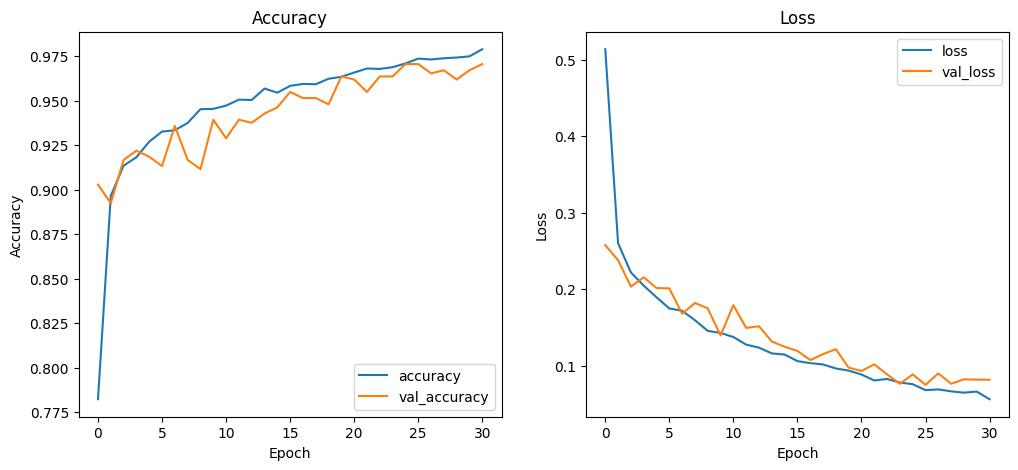
\includegraphics[width=0.85\textwidth]{Francisco/Imagenes resultados/TvsVCNN2.png} 
    \caption{Gráfica \textit{Training vs Validation} de modelo \textit{Transfer Learning} con \textit{VGG16}}
\end{figure}

\newpage

La matriz de confusión para esta CNN con modelo base \textit{VGG16} dio el resultado siguiente:

\begin{figure}[H]
    \centering
    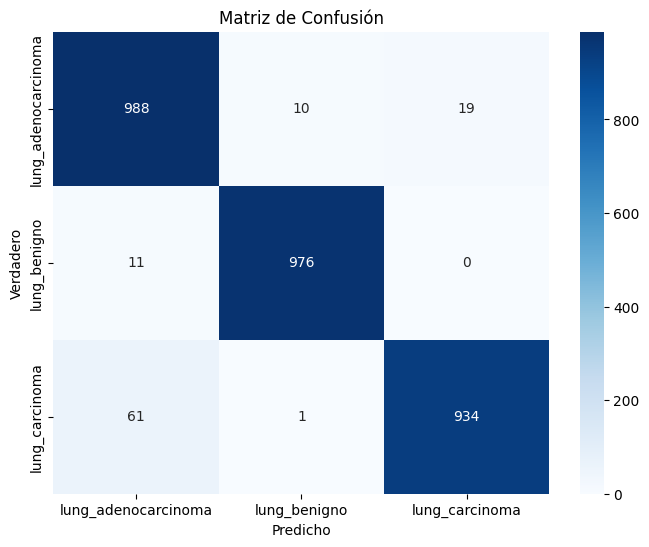
\includegraphics[width=0.65\textwidth]{Francisco/Imagenes resultados/CMCNN2.png} 
    \caption{Matriz de confusión de modelo \textit{Transfer Learning} con \textit{VGG16}}
\end{figure}

Se generó el reporte de clasificación, el resultado fue el siguiente:

\begin{table}[H]
    \centering
    \begin{tabular}{l c c c c}

         & precision & recall & f1-score & support \\
        \\
        lung\_adenocarcinoma & 0.93 & 0.97 & 0.95 & 1017 \\
        lung\_benigno & 0.99 & 0.99 & 0.99 & 987 \\
        lung\_carcinoma & 0.98 & 0.94 & 0.96 & 996 \\
        \\
        accuracy &  &  & 0.97 & 3000 \\
        macro avg & 0.97 & 0.97 & 0.97 & 3000 \\
        weighted avg & 0.97 & 0.97 & 0.97 & 3000
    
    \end{tabular}
    \caption{Reporte de clasificación de modelo \textit{Transfer Learning} con \textit{VGG16}}
\end{table}

\subsubsection{\textit{Transfer Learning} con \textit{ResNetRS101}}

Este modelo tardó también 31 épocas en entrenarse. Como con los modelos anteriores de CNN se ejecutó la siguiente celda de código para medir el \textit{accuracy} del modelo:

\lstset{
    language=Python,
    basicstyle=\ttfamily\footnotesize,
    keywordstyle=\color{blue},
    commentstyle=\color{gray},
    stringstyle=\color{green!60!black},
    numberstyle=\tiny\color{gray},
    numbers=left,
    breaklines=true,
    frame=single,
    captionpos=b,
    tabsize=4,
    showspaces=false,
    showstringspaces=false,
    showtabs=false
}

\begin{lstlisting}[caption={Código para la impresión del \textit{accuracy} del modelo}]
# Evaluamos el modelo
loss, accuracy = model.evaluate(val_ds)
print(f"Accuracy: {accuracy}")
\end{lstlisting}

\lstset{
    basicstyle=\ttfamily\footnotesize,    % Mantener la fuente monoespaciada
    backgroundcolor=\color{white},        % Fondo blanco
    keywordstyle=\color{black},           % Palabras clave en negro
    commentstyle=\color{black},           % Comentarios en negro
    stringstyle=\color{black}             % Cadenas en negro
}

\begin{lstlisting}[caption={Impresión \textit{accuracy} del modelo}]
Accuracy: 0.6293333172798157
\end{lstlisting}

\newpage

Para este modelo de CNN, se graficó igualmente \textit{Training vs Validation} para las medidas de \textit{accuracy} y \textit{loss}, resultando lo siguiente: 

\begin{figure}[H]
    \centering
    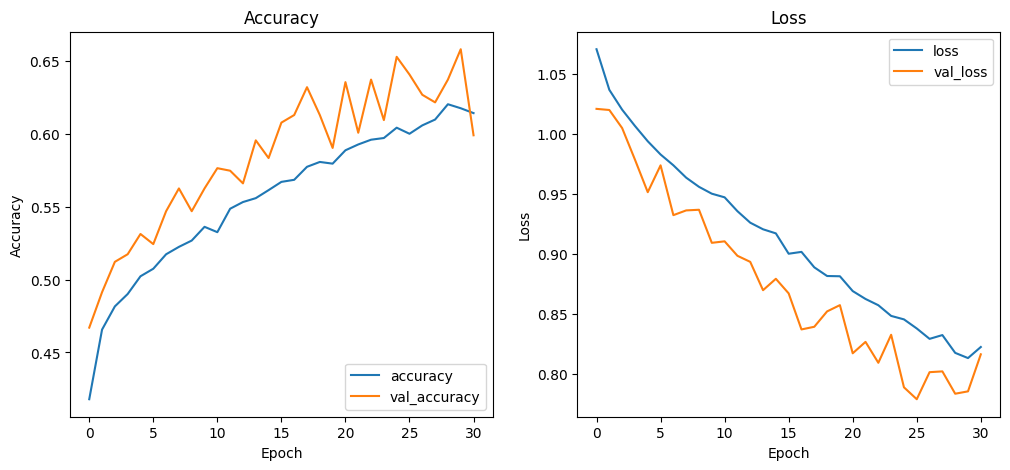
\includegraphics[width=0.85\textwidth]{Francisco/Imagenes resultados/TvsVCNN3.png} 
    \caption{Gráfica \textit{Training vs Validation} de modelo \textit{Transfer Learning} con \textit{ResNetRS101}}
\end{figure}

La matriz de confusión para este modelo de \textit{Transfer Learning} con \textit{ResNetRs101} fue la siguiente:

\begin{figure}[H]
    \centering
    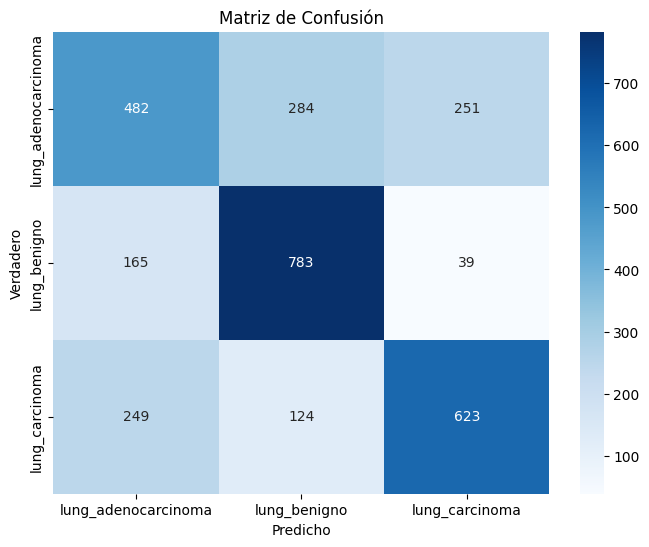
\includegraphics[width=0.65\textwidth]{Francisco/Imagenes resultados/CMCNN3.png} 
    \caption{Matriz de confusión de modelo \textit{Transfer Learning} con \textit{ResNetRs101}}
\end{figure}

\newpage

Y por último el reporte de clasificación de este modelo fue el siguiente:

\begin{table}[H]
    \centering
    \begin{tabular}{l c c c c}

         & precision & recall & f1-score & support \\
        \\
        lung\_adenocarcinoma & 0.54 & 0.47 & 0.50 & 1017 \\
        lung\_benigno & 0.66 & 0.79 & 0.72 & 987 \\
        lung\_carcinoma & 0.68 & 0.63 & 0.65 & 996 \\
        \\
        accuracy &  &  & 0.63 & 3000 \\
        macro avg & 0.63 & 0.63 & 0.63 & 3000 \\
        weighted avg & 0.63 & 0.63 & 0.62 & 3000
    
    \end{tabular}
    \caption{Reporte de clasificación de modelo \textit{Transfer Learning} con \textit{ResNetRs101}}
\end{table}

\subsubsection{\textit{Fine Tuning} con \textit{ResNetRS101}}

Este modelo tardó 9 épocas en entrenarse y demoró ligeramente más al ser un modelo con un mayor número de parámetros. Se ejecutó la siguiente celda de código para medir el accuracy del modelo: 

\lstset{
    language=Python,
    basicstyle=\ttfamily\footnotesize,
    keywordstyle=\color{blue},
    commentstyle=\color{gray},
    stringstyle=\color{green!60!black},
    numberstyle=\tiny\color{gray},
    numbers=left,
    breaklines=true,
    frame=single,
    captionpos=b,
    tabsize=4,
    showspaces=false,
    showstringspaces=false,
    showtabs=false
}

\begin{lstlisting}[caption={Código para la impresión del \textit{accuracy} del modelo}]
# Evaluamos el modelo
loss, accuracy = model.evaluate(val_ds)
print(f"Accuracy: {accuracy}")
\end{lstlisting}

\lstset{
    basicstyle=\ttfamily\footnotesize,    % Mantener la fuente monoespaciada
    backgroundcolor=\color{white},        % Fondo blanco
    keywordstyle=\color{black},           % Palabras clave en negro
    commentstyle=\color{black},           % Comentarios en negro
    stringstyle=\color{black}             % Cadenas en negro
}

\begin{lstlisting}[caption={Impresión \textit{accuracy} del modelo}]
Accuracy: 0.7236666679382324
\end{lstlisting}

Las gráficas de \textit{Training vs Validation} para las medidas \textit{accuracy} y \textit{loss} de este modelo fueron las siguientes:

\begin{figure}[H]
    \centering
    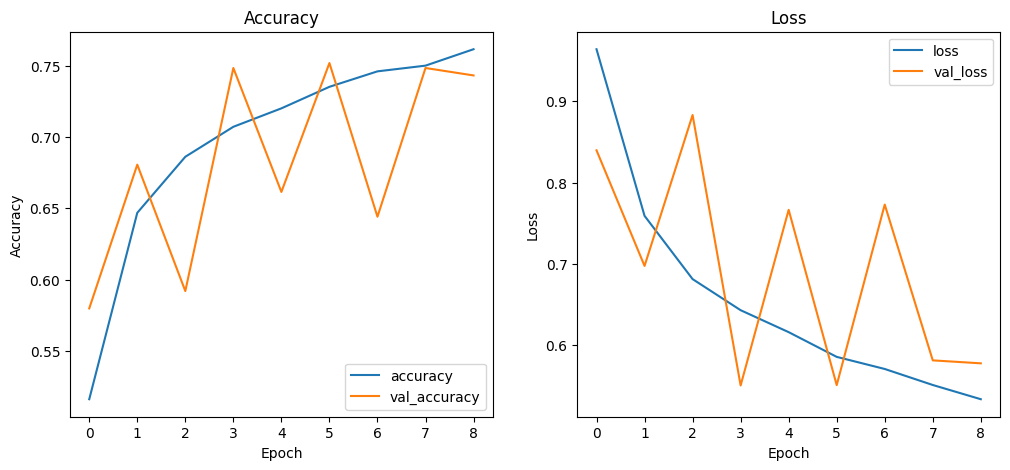
\includegraphics[width=0.85\textwidth]{Francisco/Imagenes resultados/TvsCNN4.png} 
    \caption{Gráfica \textit{Training vs Validation} de modelo \textit{Fine Tuning} con \textit{ResNetRS101}}
\end{figure}

\newpage

La matriz de confusión de este modelo de \textit{Fine Tuning} fue la siguiente:

\begin{figure}[H]
    \centering
    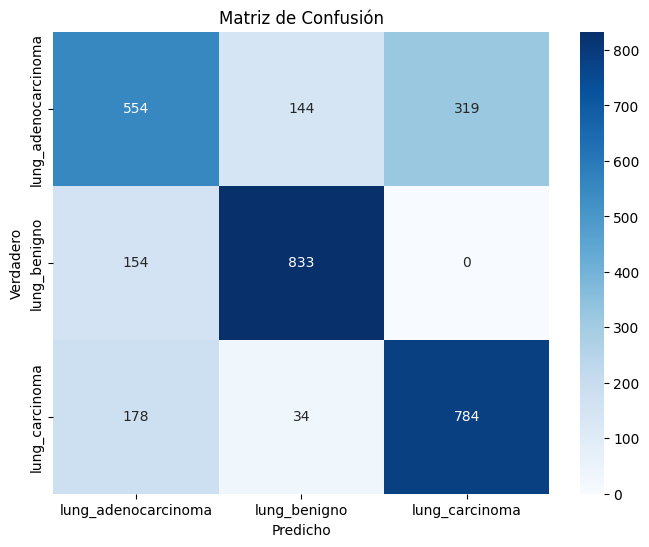
\includegraphics[width=0.65\textwidth]{Francisco/Imagenes resultados/CMCNN4.png} 
    \caption{Matriz de confusión de modelo \textit{Fine Tuning} con \textit{ResNetRs101}}
\end{figure}

El reporte de clasificación de este modelo fue el siguiente: 

\begin{table}[H]
    \centering
    \begin{tabular}{l c c c c}

         & precision & recall & f1-score & support \\
        \\
        lung\_adenocarcinoma & 0.63 & 0.54 & 0.58 & 1017 \\
        lung\_benigno & 0.82 & 0.84 & 0.83 & 987 \\
        lung\_carcinoma & 0.71 & 0.79 & 0.75 & 996 \\
        \\
        accuracy &  &  & 0.72 & 3000 \\
        macro avg & 0.72 & 0.73 & 0.72 & 3000 \\
        weighted avg & 0.72 & 0.72 & 0.72 & 3000
    
    \end{tabular}
    \caption{Reporte de clasificación de modelo \textit{Fine Tuning} con \textit{ResNetRs101}}
\end{table}

\subsubsection{Propuesta de CNN}

Esta última CNN tardó 15 épocas en entrenarse. Como con todos los modelos anteriores, se ejecutó la siguiente celda de código para calcular el \textit{accuracy} del modelo:

\lstset{
    language=Python,
    basicstyle=\ttfamily\footnotesize,
    keywordstyle=\color{blue},
    commentstyle=\color{gray},
    stringstyle=\color{green!60!black},
    numberstyle=\tiny\color{gray},
    numbers=left,
    breaklines=true,
    frame=single,
    captionpos=b,
    tabsize=4,
    showspaces=false,
    showstringspaces=false,
    showtabs=false
}

\begin{lstlisting}[caption={Código para la impresión del \textit{accuracy} del modelo}]
# Evaluamos el modelo
loss, accuracy = model.evaluate(val_ds)
print(f"Accuracy: {accuracy}")
\end{lstlisting}

\lstset{
    basicstyle=\ttfamily\footnotesize,    % Mantener la fuente monoespaciada
    backgroundcolor=\color{white},        % Fondo blanco
    keywordstyle=\color{black},           % Palabras clave en negro
    commentstyle=\color{black},           % Comentarios en negro
    stringstyle=\color{black}             % Cadenas en negro
}

\begin{lstlisting}[caption={Impresión \textit{accuracy} del modelo}]
Accuracy: 0.9129999876022339
\end{lstlisting}

\newpage

Igualmente se generaron las gráficas \textit{Training vs Validation} para este modelo, generando lo siguiente:

\begin{figure}[H]
    \centering
    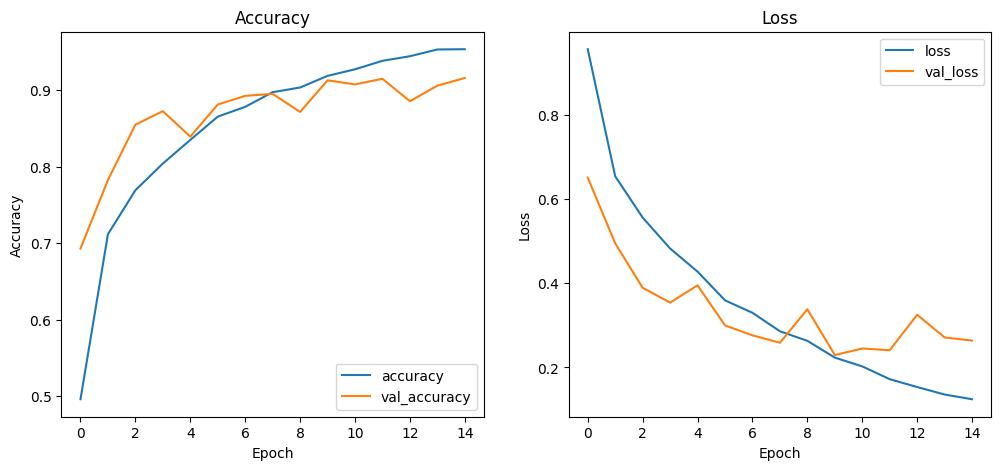
\includegraphics[width=0.85\textwidth]{Francisco/Imagenes resultados/TvsVCnn5.png} 
    \caption{Gráfica \textit{Training vs Validation} del modelo de CNN propuesto}
\end{figure}

La matriz de confusión del modelo propuesto fue la siguiente: 

\begin{figure}[H]
    \centering
    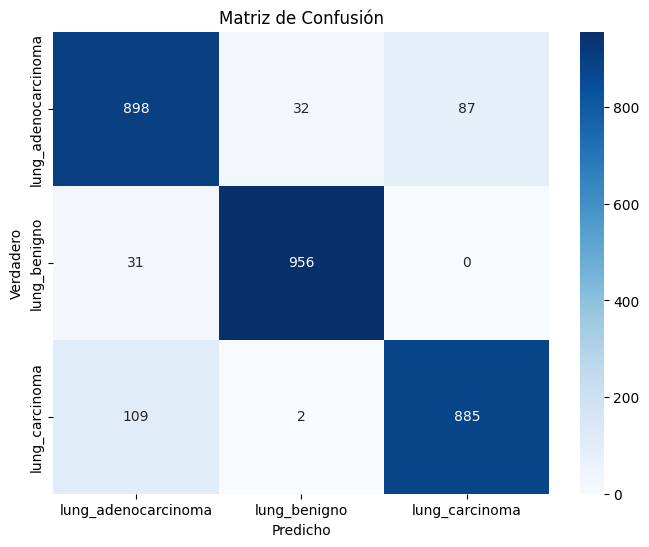
\includegraphics[width=0.65\textwidth]{Francisco/Imagenes resultados/CMCNN5.png} 
    \caption{Matriz de confusión deL modelo de CNN propuesto}
\end{figure}

\newpage

Y por último el reporte de clasificación fue el siguiente:

\begin{table}[H]
    \centering
    \begin{tabular}{l c c c c}

         & precision & recall & f1-score & support \\
        \\
        lung\_adenocarcinoma & 0.87 & 0.88 & 0.87 & 1017 \\
        lung\_benigno & 0.97 & 0.97 & 0.97 & 987 \\
        lung\_carcinoma & 0.91 & 0.89 & 0.90 & 996 \\
        \\
        accuracy &  &  & 0.91 & 3000 \\
        macro avg & 0.91 & 0.91 & 0.91 & 3000 \\
        weighted avg & 0.91 & 0.91 & 0.91 & 3000
    
    \end{tabular}
    \caption{Reporte de clasificación del modelo de CNN propuesto }
\end{table}

Para finalizar el apartado de resultados de la clasificación en este proyecto, se propone una tabla comparativa de los promedios de las diferentes métricas en los reportes de clasificación de los modelos utilizados a lo largo de esta sección.

\begin{table}[H]
    \centering
    \begin{tabular}{lcccc}
        \toprule
        Modelo              & Accuracy & Precision & Recall & F1-score \\
        \midrule
        SVC                 & 0.88 & 0.88 & 0.88 & 0.88 \\
        Regresión Logística & 0.68 & 0.68 & 0.69 & 0.68 \\
        XGBClassifier       & 0.90 & 0.90 & 0.90 & 0.90 \\
        TL MobileNetV2      & \textbf{0.99} & \textbf{0.99} & \textbf{0.99} & \textbf{0.99} \\
        TL VGG16            & \textbf{0.97} & \textbf{0.97} & \textbf{0.97} & \textbf{0.97} \\
        TL ResNetRS101      & 0.63 & 0.63 & 0.63 & 0.63 \\
        FT ResNetRS101      & 0.72 & 0.72 & 0.73 & 0.72 \\
        CNN propuesta       & 0.91 & 0.91 & 0.91 & 0.91 \\
        \bottomrule
    \end{tabular}
    \caption{Tabla comparativa de métricas de los modelos}
    \label{tabla:resultados_modelos}
\end{table}